\documentclass[12pt, twoside]{article}
\usepackage[letterpaper, margin=1in, headsep=0.2in]{geometry}
\setlength{\headheight}{0.6in}
%\usepackage[english]{babel}
\usepackage[utf8]{inputenc}
\usepackage{microtype}
\usepackage{amsmath}
\usepackage{amssymb}
%\usepackage{amsfonts}
\usepackage{siunitx} %units in math. eg 20\milli\meter
\usepackage{yhmath} % for arcs, overparenth command
\usepackage{tikz} %graphics
\usetikzlibrary{quotes, angles}
\usepackage{graphicx} %consider setting \graphicspath{{images/}}
\usepackage{parskip} %no paragraph indent
\usepackage{enumitem}
\usepackage{multicol}
\usepackage{venndiagram}

\usepackage{fancyhdr}
\pagestyle{fancy}
\fancyhf{}
\renewcommand{\headrulewidth}{0pt} % disable the underline of the header
\raggedbottom
\hfuzz=2mm %suppresses overfull box warnings

\usepackage{hyperref}

\fancyhead[LE]{\thepage}
\fancyhead[RO]{\thepage \\ Name: \hspace{4cm} \,\\}
\fancyhead[LO]{BECA / Dr. Huson / Geometry\\*  Unit 1: Segments, length, and area\\* 19 Sept 2022}

\begin{document}

\subsubsection*{1.9 Homework: Rounding and circle area} 
\begin{enumerate}
\item The $\triangle DEF$ has an area $A=54$ and base $DE=12$.
  \begin{multicols}{2}
    Find its height, starting with an equation. \\[0.5cm]
    $\displaystyle A = \frac{1}{2} bh = 54$ \vspace{2cm}
      \begin{flushright}
      \begin{tikzpicture}[scale=.635]
        %\draw[help lines] (-1,-1) grid (9,6);
        \draw[thick, ->] (-1.2,0) -- (9.4,0) node [below right] {$x$};
        \draw[thick, ->] (0,-1.2)--(0,6.4) node [left] {$y$};
        \draw[<->, thick] (0.5,1)--(0.5,5);
        \draw[thick] (2,1)--(7,1)--(1,5)--cycle;
        \draw[dashed] (7,1)--(6,5)--(1,5);
        \draw[fill] (2,1) circle [radius=0.05] node[below] {$D$};
        \draw[fill] (7,1) circle [radius=0.05] node[below] {$E$};
        \draw[fill] (1,5) circle [radius=0.05] node[above right] {$F$};
        \node at (4.5,1)[below]{$12$};
        \node at (0.5,3)[right]{$h$};
      \end{tikzpicture}
      \end{flushright}
  \end{multicols}

\item Given circle $O$ with area $A=49 \pi$ square centimeters.
  \begin{multicols}{2}
  \raggedcolumns
  Find the radius of circle, $OP$. Start with the formula\\[0.5cm]
  $A = \pi r^2 = 49 \pi$ \vspace{1.7cm}
    \begin{tikzpicture}[scale=1]
      \draw (0,0) circle[radius=3];
      \draw[thick]
      (0:3) node[right] {$P$}--
      (0,0) node[below] {$O$};
      \draw (1.5,0) node[below] {$?$};
    \end{tikzpicture}
  \end{multicols}

\item Mark each statement true of false.
\begin{enumerate}[itemsep=0.3cm]
  \item T \quad F \qquad 3.14 is the exact value of $\pi$
  \item T \quad F \qquad $4\pi$ is the area of a circle with radius 2 in terms of $\pi$
  \item T \quad F \qquad $C = 10\pi \approx 31.4$ is an approximation
  \item T \quad F \qquad $3\sqrt{2}$ is an exact value
  \item T \quad F \qquad $0.707$ is an approximation to the \emph{nearest thousandth} for $\displaystyle \frac{1}{\sqrt{2}}$
  \item T \quad F \qquad Rounding 10.498 to the nearest whole number should round up because since 9 is more than 5, first you round to 10.5, then that rounds up to 11.
\end{enumerate}



\item Find the length of the base of a triangle with area $A=78$ and height $h=20$. Express your result as a decimal. Start with the form (use $b$ or $x$): \\[0.5cm]
$A = \frac{1}{2} \times b \times h = 78$
  \begin{flushright}
  \begin{tikzpicture}[scale=1.25]
    \draw[thick] (0,0)--(3,0)--(2.5,3.5)--cycle;
    \node at (3.3, 1.5){20};
    \node at (1.5, -0.5){$?$};
    \node at (1.75, 1){$A = 78$};
  \end{tikzpicture}
  \end{flushright}

\item Find the area of the given circle $Q$ with radius $r=10$ centimeters.
  \begin{multicols}{2}
  \raggedcolumns
  Start with the formula\\[0.5cm]
  $A = \pi r^2$ 
  \begin{enumerate}
    \item State the area in terms of $\pi$ \vspace{1.7cm}
    \item Now round to the nearest hundredth
  \end{enumerate}
    \begin{tikzpicture}[scale=1]
      \draw (0,0) circle[radius=3];
      \draw[thick]
      (0:3) node[right] {$P$}--
      (0,0) node[below] {$Q$};
      \draw (1.5,0) node[below] {$10$};
    \end{tikzpicture}
  \end{multicols}

\item Find the base of a rectangle with area $A=16.8$ and height $h=4.8$, expressed as a decimal. First write an equation substituting the given values in the area formula.
  \begin{flushright}
  \begin{tikzpicture}[scale=1.25]
    \draw[thick] (0,0)--(3,0)--(3,3.5)--(0,3.5)--cycle;
    \node at (3.5, 2){$4.8$};
    \node at (1.5, -0.5){$x$};
    \node at (1.5, 2){$A = 16.8$};
  \end{tikzpicture}
  \end{flushright}

\item Find the radius and circumference of circle $O$ with diameter $D=14$ centimeters.
  \begin{multicols}{2}
  \raggedcolumns
  \begin{enumerate}
    \item Write down the radius. \vspace{1.2cm}
    \item State the circumference in terms of $\pi$ \vspace{1cm}
    \item Express the circumference as a decimal, rounding to the nearest tenth.
  \end{enumerate}
  \columnbreak
    \begin{tikzpicture}[scale=1]
      \draw (0,0) circle[radius=3];
      \draw[thick] (0:3)--(0,0)--(-3,0);
      \draw[fill] (0,0) circle [radius=0.05] node[below]{$O$};
      \draw (1.5,0) node[below] {$r$};
    \end{tikzpicture}
  \end{multicols}

\newpage
\item A parallelogram is shown on the $x$-$y$ plane having a base $b=4$ and height $h=3$. 
  \begin{multicols}{2}
    Find its area, showing the calculation.
      \begin{flushright}
      \begin{tikzpicture}[scale=.635]
        \draw[help lines] (-1,-1) grid (9,6);
        \draw[thick, ->] (-1.2,0) -- (9.4,0) node [below right] {$x$};
        \draw[thick, ->] (0,-1.2)--(0,6.4) node [left] {$y$};
        \draw[<->, thick] (1.5,1)--(1.5,4);
        \draw[thick] (2,1)--(6,1)--(7,4)--(3,4)--cycle;
        \node at (4,1)[below]{$4$};
        \node at (1.5,2.5)[left]{$3$};
      \end{tikzpicture}
      \end{flushright}
  \end{multicols} 

\item The $\triangle ABC$ is shown below with $A(2,1)$, $B(7,1)$, and $C(1,5)$. The length of the base of the triangle is $AB=5$.
  \begin{multicols}{2}
    \begin{enumerate}
      \item Find the height $h$.
      \item Find its area, showing the calculation. \vspace{2cm}
      \end{enumerate}
      \begin{flushright}
      \begin{tikzpicture}[scale=.635]
        \draw[help lines] (-1,-1) grid (9,6);
        \draw[thick, ->] (-1.2,0) -- (9.4,0) node [below right] {$x$};
        \draw[thick, ->] (0,-1.2)--(0,6.4) node [left] {$y$};
        \draw[<->, thick] (0.5,1)--(0.5,5);
        \draw[thick] (2,1)--(7,1)--(1,5)--cycle;
        \draw[dashed] (7,1)--(6,5)--(1,5);
        \draw[fill] (2,1) circle [radius=0.05] node[below] {$A$};
        \draw[fill] (7,1) circle [radius=0.05] node[below] {$B$};
        \draw[fill] (1,5) circle [radius=0.05] node[above right] {$C$};
        \node at (4.5,1)[below]{$5$};
        \node at (0.5,3)[right]{$h$};
      \end{tikzpicture}
      \end{flushright}
  \end{multicols} 

  \item Rectangle $ABCD$ has area $A=15$ and base $b=6$ but unknown height. Write an equation then solve. Start with this form (for the unknown, use $h$, $x$, or $BC$) and state your answer as a fraction: \\[0.5cm]
$A = b \times h = 15$
  \begin{flushright}
  \begin{tikzpicture}[scale=1.25]
    \draw[thick] (0,0)--(4.5,0)--(4.5,2)--(0,2)--cycle;
    \draw[fill] (0,0) circle [radius=0.05] node[left]{$A$};
    \draw[fill] (4.5,0) circle [radius=0.05] node[right]{$B$};
    \draw[fill] (4.5,2) circle [radius=0.05] node[right]{$C$};
    \draw[fill] (0,2) circle [radius=0.05] node[left]{$D$};
    \node at (5, 1){?};
    \node at (2.25, -0.5){$6$};
    \node at (2.25, 1){$A = 15$};
  \end{tikzpicture}
  \end{flushright}

  \newpage
  \item Find the area of the shape shown below composed of a rectangle and circular cap. Leave your answer as an exact value in terms of $\pi$.
    \begin{flushright}
    \begin{tikzpicture}[scale=.635]
      \draw[help lines] (-2,-1) grid (8,7);
      \draw[thick, ->] (-2.2,0) -- (8.4,0) node [below right] {$x$};
      \draw[thick, ->] (0,-1.2)--(0,7.4) node [left] {$y$};
      \draw[thick] (1,1)--(7,1)--(7,3)--(1,3)--cycle;
      %\draw[thick] (3,4) arc (90:270:1);
      \draw[thick] (7,3) arc (0:180:3);
    \end{tikzpicture}
    \end{flushright}
  
  \item Find the \emph{perimeter} of the shape shown below composed of a rectangle and circular cap. Leave your answer as an exact value in terms of $\pi$.
  \begin{flushright}
  \begin{tikzpicture}[scale=.635]
    \draw[help lines] (-1,-1) grid (7,7);
    \draw[thick, ->] (-1.2,0) -- (7.4,0) node [below right] {$x$};
    \draw[thick, ->] (0,-1.2)--(0,7.4) node [left] {$y$};
    \draw[thick] (1,1)--(5,1)--(5,4)--(1,4)--cycle;
    %\draw[thick] (3,4) arc (90:270:1);
    \draw[thick] (5,4) arc (0:180:2);
  \end{tikzpicture}
  \end{flushright}
  
  \item Find the area of the shape shown below composed of a rectangle and a semi-circle.
    \begin{flushright}
    \begin{tikzpicture}[scale=.635]
      \draw[help lines] (-2,-1) grid (10,7);
      \draw[thick, ->] (-2.2,0) -- (10.4,0) node [below right] {$x$};
      \draw[thick, ->] (0,-1.2)--(0,7.4) node [left] {$y$};
      \draw[thick] (1,1)--(6,1)--(6,5)--(1,5)--cycle;
      \draw[thick] (6,1) arc (-90:90:2);
    \end{tikzpicture}
  \end{flushright}
    
  \item Given the circle $A$ with radius $r=3$. Leave exact answers, in terms of $\pi$.
    \begin{multicols}{2}
      \begin{enumerate}
        \item Find the circumference of circle $A$. \vspace{1cm}
        \item Find the area of the circle.\vspace{2cm}
      \end{enumerate}
      \begin{flushright}
      \begin{tikzpicture}[scale=.9]
        \draw (0,0) circle [radius=3];
        \draw[fill] (0,0) circle [radius=0.05] node[below right]{$A$};
        \draw[thick, -{>[scale=1.5]}] (0,0)--(30:3);
        \node at (2,0.5){$r=3$};
        \clip (0,0) circle [radius=3];
          \draw[help lines] (-4,-4) grid (4,4);
      \end{tikzpicture}
    \end{flushright}
    \end{multicols}
  
  
  \newpage
  \item One side of the $\triangle ABC$ has a length $AB=8$. The triangle's area is 44. Find the length of the altitude $h$ of the triangle to vertex $C$ and perpendicular to side $\overline{AB}$. \par
    \begin{tikzpicture}[scale=1, rotate=-40]
      \draw[thick]
        (2,0)node[below]{$A$}--
        (8,0)node[below]{$B$}--
        (5,3)node[above]{$C$} --(2,0);
      \draw[dashed] (5,0)--(5,3);
      \draw (5,0)++(0.3,0)--++(0,0.3)--+(-0.3,0);
      \node at (5,1)[right]{$h=?$};
      \node at (5,0)[below left]{$8$};
    \end{tikzpicture}
  
  \item One side of the $\triangle ABC$ has a length $AB=12$. The triangle's area is 60. Find the length of the altitude $h$ of the triangle to vertex $C$ and perpendicular to side $\overline{AB}$. \par
  \begin{tikzpicture}[scale=0.9, rotate=30]
    \draw[thick]
      (2,0)node[below]{$A$}--
      (8,0)node[below]{$B$}--
      (5,3)node[above]{$C$} --(2,0);
    \draw[dashed] (5,0)--(5,3);
    \draw (5,0)++(0.3,0)--++(0,0.3)--+(-0.3,0);
    \node at (5.2,1.5)[right]{$h=?$};
    \node at (5,-0.5)[below left]{$12$};
  \end{tikzpicture}
  
  \item Find the area of $\triangle ABC$ shown below (not actual size) with $m\angle C=90^\circ$ and the lengths of the triangle's sides as $a=3$, $b=4$, and $c=5$. 
  \begin{flushright}
  \begin{tikzpicture}[scale=1.4]
    \draw[thick]
    (0,0)node[left]{$A$}--
    (4,0)node[below right]{$C$}--
    (4,2.31)node[right]{$B$}--cycle;
    \draw (4,0)++(-0.3,0)--++(0,0.3)--+(0.3,0);
    \node at (2,0)[below]{$b=4$};
    \node at (4,1.2)[right]{$a=3$};
    \node at (1.8,1.4)[above]{$c=5$};
  \end{tikzpicture}
  \end{flushright}
  \vspace{1cm}
  
  \item Find the area of $\triangle ABC$ shown below (not actual size) with $m\angle C=90^\circ$ and the lengths of the triangle's sides as $a=50$, $b=87$, and $c=100$. \par \medskip
    \begin{tikzpicture}[scale=1.4]
      \draw[thick]
      (0,0)node[left]{$A$}--
      (4,0)node[below right]{$C$}--
      (4,2.31)node[right]{$B$}--cycle;
      \draw (4,0)++(-0.3,0)--++(0,0.3)--+(0.3,0);
      \node at (2,0)[below]{$b=87$};
      \node at (4,1.2)[right]{$a=50$};
      \node at (1.8,1.4)[above]{$c=100$};
    \end{tikzpicture}
  
  \item The compound shape shown below is composed of a square with side length 5 cm and a triangle with base 2 cm. Find the total area of the combined shape.
    \vspace{1cm} 
    \begin{flushleft}
    \begin{tikzpicture}
      \draw[thick] (0,0)--(7,0)--(5,5)--(0,5)--cycle;
      \draw[dashed] (5,0)--(5,5);
      \node at (6, -0.5){2};
      \node at (2.5, -0.5){5};
      \node at (-0.5, 2.5){5};
    \end{tikzpicture}
    \end{flushleft} \vspace{1cm}
  \item Repeat the calculation for the figure above using the trapezoid area formula. \vspace{1cm}
  
  \item On the grid below, accurately draw and label two adjacent squares, one with a side length of 4 cm, the other with a side length of 3 cm. The grid is in centimeters. \par \medskip
    Find the area $A$ and perimeter $P$ of combined shape.
    \begin{flushleft}
      \begin{tikzpicture}[scale=0.2]
        \draw[help lines] (-4,-3) grid (5,3);
        %\draw[thick, ->] (-2.2,0) -- (10.4,0) node [below right] {$x$};
        %\draw[thick, ->] (0,-2.2)--(0,10.4) node [left] {$y$};
        %\draw (0,0) circle [radius=3] node[below]{$C$};
        %\draw[fill] (0,0) circle [radius=0.05];
        %\draw[thick, -] (-3,-3)--(4,-3);
      \end{tikzpicture}
    \end{flushleft}
  
  \item On the graph, draw polygon ABCDEF with vertices A(1, 1), B(1, 4), C(3, 4), D(3, 7), E(8, 7), and F(8, 1). Find the perimeter and the area of the polygon.
  \begin{flushleft}
    \begin{tikzpicture}[scale=.2]
      \draw[help lines] (0,0) grid (10,10);
      \draw[thick, ->] (0,0) -- (10.4,0) node [below right] {$x$};
      \draw[thick, ->] (0,0)--(0,10.4) node [right] {$y$};
      \foreach \x in {1,...,10}
      \draw[shift={(\x,0)}] (0pt,-3pt)--(0pt,3pt) node[below=5pt] {$\x$};
      \foreach \y in {1,...,10}
      \draw[shift={(0,\y)}] (-3pt,0pt)--(3pt,0pt) node[left=5pt] {$\y$};
    \end{tikzpicture}
    \end{flushleft}
  
  \item Draw and label a triangle $\triangle ABC$ with base $\overline{AB}$ 8 centimeters long and altitude of 5 centimeters. (show the altitude as a dotted line, and make sure it is perpendicular to the base) 
  
  

\end{enumerate}
\end{document}